\section{Metodologia SFC: Uma breve introdução}

A presente seção ter por objetivo apresentar as etapas e procedimentos da metodologia \textit{Stock Flow Consistent} (adiante SFC\footnote{Cabe aqui destacar que tal nomenclatura decorre do trabalho de })\footnote{Para uma análise mais pormenorizada das linhagens da abordagem SFC, ver \textcite{caverzasi_stock-flow_2013}.}. De forma bastante sucinta, tal metodologia é composta de três procedimentos: (i) determinhação da estrutura contábil; (ii) exposição das equações comportamentais e; (iii) solução. Dito isso, a figura \ref{Resuminho} pretende resumir as etapas mencionadas e explicitar a diferença entre a abordagem SFC de um modelo SFC. 

\begin{figure}[htb]
	\caption{Resumo esquemático da Metodologia SFC}
	\label{Resuminho}
	\centering
	\begin{tikzpicture}
	[node distance = 1cm, auto,font=\footnotesize,
	% STYLES
	every node/.style={node distance=3cm},
	% The comment style is used to describe the characteristics of each force
	comment/.style={rectangle, inner sep= 5pt, text width=4cm, node distance=0.25cm, font=\scriptsize\sffamily},
	% The force style is used to draw the forces' name
	force/.style={rectangle, draw, fill=black!10, inner sep=5pt, text width=4cm, text badly centered, minimum height=1.2cm, font=\bfseries\footnotesize\sffamily}] 
	
	% Draw forces
	\node [force] (rivalry) {Equações comportamentais};
	\node [force, above of=rivalry, fill=red!70] (substitutes) {Hipóteses};
	\node [force, text width=3cm, dashed, left=1.5cm of substitutes,fill=blue!50] (state) {Metodologia SFC};
	\node [force, left=1cm of rivalry] (suppliers) {Estrutura contábil};
	\node [force, right=1cm of rivalry] (users) {Resolução};
	\node [force, right=1cm of substitutes, dashed, fill=purple!50 ] (PK) {Modelo \\SFC};
	%	\node [force, below of=rivalry] (entrants) {Threat of new entrants};
	
	%%%%%%%%%%%%%%%
	% Change data from here
	
	% RIVALRY
	\node [comment, below=0.25 of rivalry] (comment-rivalry) {Cambridge\\
		Kaleckiano\\
		\textbf{Supermultiplicador Sraffiano}};
	
	
	% SUBSTITUTES
	%\node [comment, right=0.25 of substitutes] {};
	
	% USERS
	\node [comment, below=0.25 of users] {Analítico\\
		\textbf{Simulação}};
	
	% NEW ENTRANTS
	%	\node [comment, right=0.25 of entrants] {(+) EC vs. Microsoft};
	
	% PUBLIC POLICIES
	%	\node [comment, text width=3cm, below=0.25 of state] {(1) Estrutura contábil\\
	%	(2) Equações comportamentais\\
	%	(3) \textit{Closure} do modelo};
	
	%%%%%%%%%%%%%%%%
	
	% Draw the links between forces
	\path[->,thick] 
	(substitutes) edge (rivalry)
	(suppliers) edge (rivalry)
	(rivalry) edge (users)
	(state) edge (substitutes)
	(state) edge (suppliers)
	(substitutes) edge (PK);
	
	%(entrants) edge (comment-rivalry);
	
	\end{tikzpicture} 
	\caption*{Fonte: \textcite[p.~64, adaptado]{da_silveira_politica_2017}}

	
\end{figure}


As etapas contábeis da abordagem SFC constituem em\footnote{Esta seção não pretende expor a metodologia pormenorizadamente, mas sim expor seus procedimentos de modo a esclarecer as etapas que foram adotadas. Dito isso, a construção das matrizes a serem usadas fica a cargo da seção \ref{SecModelo}. Para uma apresentação mais gradual, ver \textcite[Capítulo 4]{da_silveira_politica_2017}.}: (i) seleção dos setores institucionais e dos ativos a serem incorporados; (ii) mapeamento das relações dos fluxos entre os mencionados setores por meio da construção da matriz de fluxos; (iii) construção da matriz dos estoques de riqueza (real e financeira) em que são contabilizadas os ativos e passivos  bem como a posição líquida de cada setor; (iv) identificação das formas que os fluxos são financiados e sua respectiva acumulação nos estoques. Desse modo, o rigor contábil adotado faz com que o grau de liberdade, ou seja arbitrariedade, do modelo diminua. 
Grosso modo, ao partir de um aparato analítico baseado em identidades macroeconômicas, surgem restrições que precisam ser seguidas.

Vale destacar que as identidades contábeis são o ponto de partida, mas não são suficientes para garantir a consistência do modelo. Para isso, é necessário que a soma da posição financeira líquida de cada setor institucional seja zero de modo que não existam ``buracos negros''. Grosso modo, tal procedimento garante que para que um setor acumule riqueza financeira, outro precisa necessariamente liquidá-la. Isto posto, conclui-se a estrutura contábil da metodologia SFC a partir das identidades macroeconômicas. 

Por mais que esta etapa é centrada na contabilidade social, isso não implica que não possua um componente teórico associado. A título de exemplo, \textcite[p.~15--16]{macedo_e_silva_peering_2011}  pontuam que estão presentes elementos pós-keynesianos: (i) os agentes econômicos são categorizados de acordo com o tipo de estoque de riqueza que possuem; (ii) os agentes celebram contratos que impactam sua riqueza e geram fluxos monetários que implicam novas mudanças na composição patrimonial desses agentes; (iii) ganhos e perdas de capital afetam o valor dos estoques que impactam na dinâmica do sistema; (iv) a composição patrimonial dos agentes e setores evolui de forma assimétrica de acordo com o grau de alavancagem, preferência
pela liquidez/risco e (v) o acúmulo de ativos e passivos pelos agentes interfere na correlação de forças da economia. 

Desse modo, por mais que a estrutura contábil parta das identidades, isso não a isenta de teoria. No entanto, por se tratar de identidades, nada de causal pode ser extraído delas. As relações de causalidade do modelo (agora modelo e não metodologia) decorrem das equações comportamentais que, respeitando a consistência, podem ser de qualquer linhagem teórica (\textit{e.g.} Kaleckiana, Sraffinana, Neoclássica, etc.). A ênfase em tratar a abordagem SFC enquanto uma metodologia decorre da flexibilidade de incluir inúmeras teorias e propostas apesar da rigidez de seus procedimentos. Apenas para elencar (e não esgotar) alguns temas caros a heterodoxia, tal abordagem permite tratar as formas de financiamento das firmas \cites{asimakopulos_kalecki_1983}{skott_finance_1988}{messori_financing_1991}; endogeneidade da moeda e importância do sistema bancário \cites{messori_financing_1991}{dow_horizontalism:_1996}{arestis_theoretical_1996}{godley_money_1999}{lavoie_note_1999}{lima_macrodynamics_2007}; endividamento, distribuição de renda e financeirização \cites{palley_inside_1996}{wolfson_irving_1996}{palley_money_1997}{palley_financial_2002}{dos_santos_revisiting_2009}{palley_inside_2010}{hein_finance-dominated_2012} e, apenas para restringir os temas; análises empíricas e proposições de política econômica \cites{godley_seven_1999}{godley_fiscal_2007}{godley_simple_2007}{arestis_income_2011}{zezza_design_2019}. 

A mesma variabilidade de temas passíveis de serem abordados pela metodologia SFC se estende para a pluralidade dos ativos e do grau de complexidade financeira de cada modelo. Uma forma de visualizar tal flexibilidade é por meio da figura \ref{Heatmap} em que são mapeados os ativos mais frequentes. No entanto, este gráfico também revela que a literatura não dá a devida atenção ao investimento residencial\footnote{Deve ser pontuada a notória exceção de \textcite{zezza_u.s._2008} em que é apresentado um modelo com imóveis em um aparato Kaleckiano mas não trata de questões envolvendo ganhos de capital ou dos determinantes do investimento residencial.}. 
\begin{figure}
    \centering
    \caption{Mapa de calor dos ativos modelados com SFC}
    \label{Heatmap}
    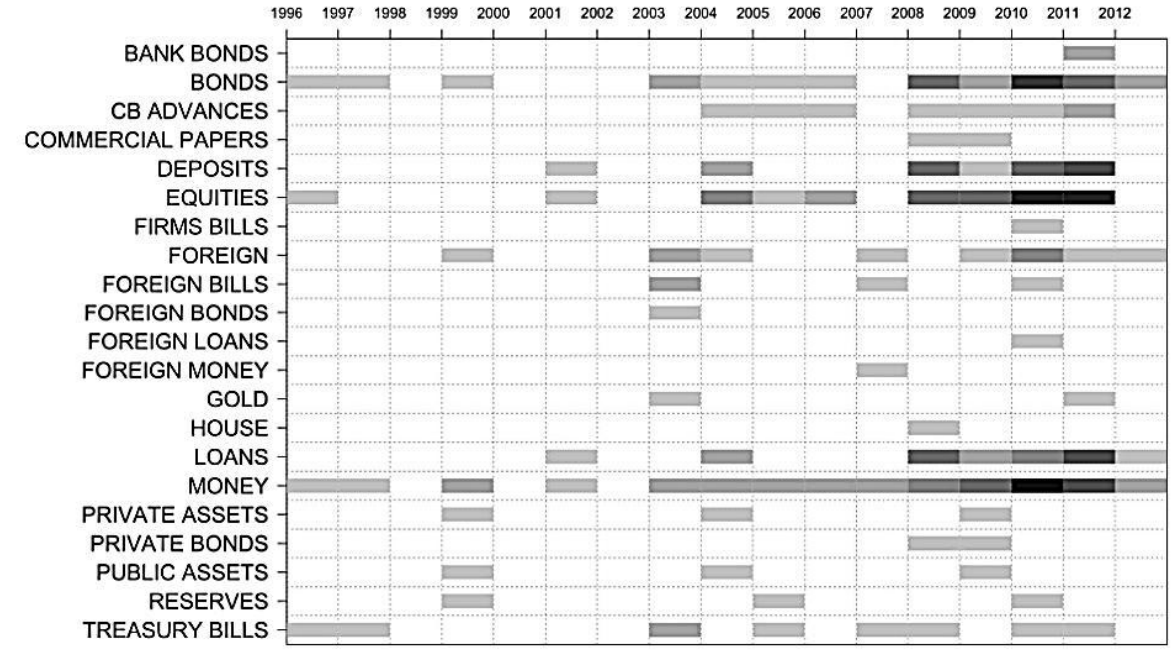
\includegraphics[width = 0.9\textwidth]{Modelo/Caverzassi_Heatmap.png}
    \caption*{\textbf{Fonte:} \textcite[p.~4]{caverzasi_stock-flow_2013}}
\end{figure}


%BREVE REVISÃO MODELOS SHIPMAN + GRÁFICO CAVERZASSI



Feitas essas ressalvas, dada a estrutura contábil e explicitadas as hipóteses (via equações comportamentais), resta seguir para a solução do modelo. Como pontuam \textcite{caverzasi_stock-flow_2013}, existem duas vias: (i) simulação e (ii) descrição. A primeira delas permite expor de forma mais clara as relações entre as variáveis de modelos mais complexos em que a solução analítica não é facilmente encontrada. No entanto, tal caminho fez com que o grau de complexidade dos modelos simulados fosse exponencializada de modo que a intuição econômica torna-se facilmente turva. Diante destas complicações, o presente capítulo prioriza a parcimônia de modo que serão incluídos apenas os elementos necessários para a narrativa. A justificativa deste procedimento decorre da maior clareza que tal modelagem frente a um menor ``realismo''. Além disso, tal postura permite encontrar soluções analíticas com maior facilidade de modo que são explicitados os parâmetros mais relevantes para as trajetórias de longo prazo. Dito isso, a seção seguinte expõe o modelo que será simulado adiante.